\documentclass[paper=a4,fontsize=11pt]{temp} % KOMA-article class
\begin{document}

\newcommand\textbox[1]{%
  \parbox{.333\textwidth}{#1}%
}

\hyphenation{ka-te-go-ri-ze}
\hyphenation{prog-ram-la-ya-bil-mek-tir}
\hyphenation{edi-le-rek}

\begin{minipage}{.2\linewidth}
   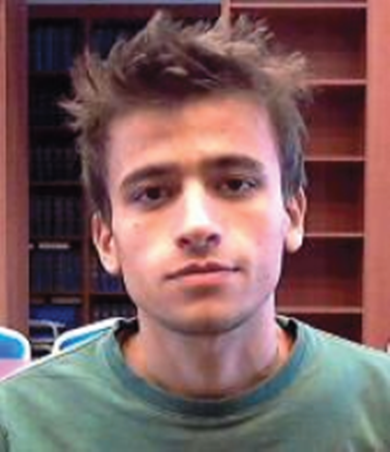
\includegraphics[width=1\textwidth]{photo}
\end{minipage}
\begin{minipage}{0.7\linewidth}
   \MyName{Fatih Çomak}
   \sepspace

\noindent\textbox{ \hfill}\textbox{\hfil \textbf{
\includegraphics[scale=0.75]{IMG/logo/mail}}\hfil}\textbox{ azeemsarwarr1@gmail.com}
\vspace{1mm}
\noindent\textbox{ \hfill}\textbox{\hfil \textbf{
\includegraphics[scale=0.75]{IMG/logo/phone}}\hfil}\textbox{ +4915224214567}
\vspace{1mm}
\noindent\textbox{ \hfill}\textbox{\hfil \textbf{
\includegraphics[scale=0.75]{IMG/logo/location}}\hfil}\textbox{ Nordhausen, Thuringia - Germany }
\vspace{1mm}
\noindent\textbox{ \hfill}\textbox{\hfil \textbf{
\includegraphics[scale=0.75]{IMG/logo/linkedin}}\hfil}\textbox{ linkedin.com/in/azeemsarwarr}
\vspace{1mm}
\noindent\textbox{ \hfill}\textbox{\hfil \textbf{
\includegraphics[scale=0.0125]{IMG/logo/github}}\hfil}\textbox{ github.com/azeem\-sarwar}

\end{minipage}

\NewPart{Bilgiler}{}
\noindent

\textbox{\textbf{Askerlik Durumu} \hfill}\textbox{\hfil Tecilli - 2022 \hfil}\textbox{\hfill}

\textbox{\textbf{Doğum Tarihi} \hfill}\textbox{\hfil 25.09.1993 \hfil}\textbox{\hfill}

\textbox{\textbf{Doğum Yeri} \hfill}\textbox{\hfil Antalya \flag{IMG/flag/tr} \hfil}\textbox{\hfill}

\NewPart{Eğitim}{}
\indent
\newline
\indent
\EducationEntry{Yıldız Teknik \"{U}niversitesi Bilgisayar Mühendisliği, Lisans}{Haziran 2020}{Diploma Notu: 2,40/4}{\%30 İngilizce eğitim.} {IMG/ytu_tr}
\newline\newline
\sepspace

\EducationEntry{Isparta Süleyman Demirel Fen Lisesi}{Haziran 2012}{Diploma Notu: 89,3/100}{} {IMG/isdfl}
\sepspace


\NewPart{Yabancı Dil}{}
\indent
\textbox{\textbf{İngilizce \flag{IMG/flag/gb}} \hfill}\textbox{\hfil Profesyonel Çalışma Yetkinliği \hfil}\textbox{\hfill}
\sepspace


\NewPart{Beceri \& Yetenekler}{}
\hspace{3mm}
\begin{minipage}[t]{0.33\textwidth} 

\begin{tabular}[t]{ l l }
\textbf{Programlama Dilleri}
\end{tabular}

\sepspace

\end{minipage}
%
\begin{minipage}[t]{0.66\textwidth} 



\begin{tabular}{lllllllllll}

\includegraphics[scale=0.035]{IMG/languages/assembly} & \textbf{Assembly} & : & Az  &  &  & 
\includegraphics[scale=0.03]{IMG/languages/htmlCss} & \textbf{HTML, CSS}  & : &  & Orta   \\
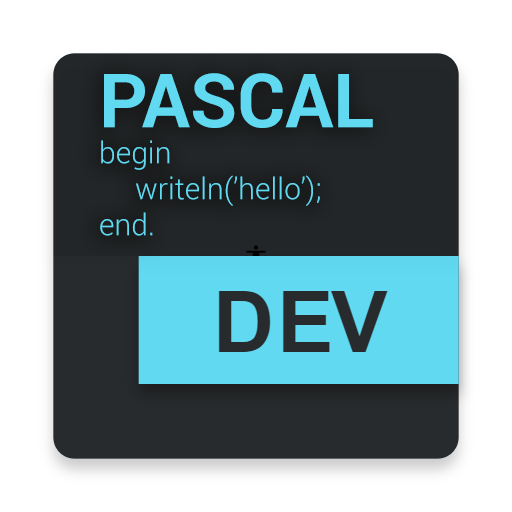
\includegraphics[scale=0.02]{IMG/languages/pascal} & \textbf{Pascal}   & : & Az  &  &  & 
\includegraphics[scale=0.075]{IMG/languages/javascript} & \textbf{JavaScript} & : &  & Az  \\

\includegraphics[scale=0.05]{IMG/languages/c} & \textbf{C}        & : & \textbf{İyi} &  &  & 
\includegraphics[scale=0.015]{IMG/languages/aspnet} & \textbf{ASP.NET}    & : &  & Az  \\

\includegraphics[scale=0.05]{IMG/languages/cplusplus} & \textbf{C++}      & : & Az  &  &  & 
\includegraphics[scale=0.03]{IMG/languages/prolog} & \textbf{Prolog}     & : &  & Az  \\

\includegraphics[scale=0.05]{IMG/languages/csharp} & \textbf{C\#}      & : & \textbf{Orta}  &  &  & 
\includegraphics[scale=0.06]{IMG/languages/sql} & \textbf{SQL}        & : &  & \textbf{Orta}   \\

\includegraphics[scale=0.05]{IMG/languages/java} & \textbf{Java}     & : & \textbf{Orta}   &  &  & 
\includegraphics[scale=0.04]{IMG/languages/groovy} & \textbf{Groovy}     & : &  & Az \\

\includegraphics[scale=0.05]{IMG/languages/python} & \textbf{Python}   & : & Az  &  &  & 
\includegraphics[scale=0.015]{IMG/languages/matlab} & \textbf{Matlab}     & : &  & Az
\end{tabular}

\end{minipage} \\\\\\


\begin{minipage}[t]{0.33\textwidth} 

\begin{tabular}[t]{ l l }
\textbf{Yetenekler}
\end{tabular}

\sepspace

\end{minipage}
%
\begin{minipage}[t]{0.66\textwidth} 



\begin{tabular}{llllll}
\textbf{Web Teknolojileri}   & : & 
\includegraphics[scale=0.04]{IMG/tech/angular} Angular, 
\includegraphics[scale=0.04]{IMG/tech/spring}Spring, 
\includegraphics[scale=0.04]{IMG/tech/hibernate} Hibernate                 &  &  &  \\
\textbf{Yapay Zeka}          & : & Makine Öğrenmesi, Uzman Sistemler          &  &  &  \\
\textbf{Programlama}         & : & C (Yapısal), OOP (Nesne Yönelimli)         &  &  &  \\
\textbf{Veritabanı Yönetimi} & : & 
\includegraphics[scale=0.02]{IMG/tech/postgresql} PostgreSQL                                 &  &  &  \\
\textbf{İşletim Sistemleri}  & : & 
\includegraphics[scale=0.03]{IMG/tech/linux} Linux                                      &  &  &  \\
\textbf{Veri Analizi}        & : & Veri Madenciliği, Big Data, Biyoenformatik &  &  & 
\end{tabular}

\end{minipage}



\NewPart{Deneyimler}{}
\indent
\newline
\indent
\workEntry{Xinerji Teknoloji Hizmetleri}{Eylül 2018 - Nisan 2019}{Part-time Developer}{Çok iplikli lojistik ERP TMAXX isimli kurumsal web uygulamasının geliştirilmesinde rol üstlendim. TMAXX, back-end için Java - Spring Boot, front-end için Angular ve server için PostgreSQL kullanılarak geliştirilmiş projedir.
Ayrıca Git kullanımı, Microservices, Docker tecrübesi edindim.} {IMG/xinerji}
\newline\newline
\sepspace

\workEntry{etcBASE Yazılım ve Bilişim Teknolojileri}{2017 Yaz Dönemi}{Staj}{Başlıca Angular olarak JavaScript frameworkleri ve Spring teknolojileri üzerine araştırmalar yapıldı, dökümantasyonlar tarandı ve karşılaştırmalar yapıldı. TypeScript SPA mimarisi analiz edildi. Bu doğrultuda sunum hazırlandı.}{IMG/etcbase}
\newline\newline
\sepspace

\workEntry{Garanti Teknoloji}{2015 Yaz Dönemi}{Staj}{HTML, CSS, (gerektiğinde) JavaScript, SQL, ASP.NET, C\# becerileri edinildi; ayrıca ASP.NET Page Life Cycle analiz edildi, client-server Data akışı araştırıldı. Edinilen web mimarisi bilgisi ışığında konsol ve form uygulamaları ile staj projesi olarak da bir demo web uygulaması geliştirildi.}{IMG/garanti}
\sepspace


\NewPart{Projeler}{}
\indent
\newline
\indent
\workEntry{Müşteri Memnuniyeti Anketi}{Temmuz 2020}{Hobi Proje}{\textbf{URL:} \emph{github.com/Sillyon/customer-satisfaction-survey} \newline
Bir anket konusu üzerinden müşteri memnuniyetini ölçen anket sunan ve GitHub üzerinde geliştirilen bir \textbf{RESTful Web API} projesidir. Puanlandırmalar baz alınarak her anket konusunun NPS skoru hesaplanır.
\newline
Back-end, Java dilinde Maven build ve Spring Boot ile yazıldı. JPA, Hibernate, Lombok, Swagger kullanıldı. Server için in-memory H2 Database seçildi. JUnit test yazıldı. Postman ve Swagger-ui'dan faydalanıldı.
Front-end ise React JS ile yazıldı.}{IMG/project/nps}

\sepspace

\workEntry{SDLC Dönüşümünde DevOps Yaklaşım }{Ağustos 2019 - Ocak 2020}{Bitirme Tezi}{\textbf{Ekip Arkadaşı:} Selahattin Gürgen\textbf{; Danışman:} Prof.Dr. Oya Kalıpsız \newline
DevOps yaklaşımı ile uçtan uca Yazılım Geliştirme Yaşam Döngüsü otomasyonu dockerize edilerek semantik versiyon yönetimi sağlandı. Sürüm notunu çıkaran \textbf{Commit Difference Finder} Plugin ve bir script geliştirildi. Git, Jira, Bitbucket, Jenkins, Groovy, Java, Linux Bash, Atlassian SDK kullanıldı. Jira'da task açılmasından ürünün canlıya alınmasına kadar olan süre saniyeler seviyesine indirildi. Esneklik sağlandı.}{IMG/project/devops}

\sepspace

\workEntry{Android Malware Detection}{Ocak 2019 - Haziran 2019}{Akademik Proje}{\textbf{Ekip Arkadaşı:} Alibek Erkabayev\textbf{; Danışman:} Arş.Gör. Alper Eğitmen
\newline
\textbf{URL:} \emph{github.com/bigalex95/androidMalwareDetectionSystem} \newline
Makine öğrenmesini Supervised kullanan, statik opcode analizine dayalı bir yaklaşım sunularak Word Embedding ve Word2Vec yöntemi kullanıldı. Apk DataSet, doğal dil olarak modellendi ve işleme, kelime vektörleri üzerinden gerçeklendi. Ön-işleme ve hashleme için C++, Python kullanıldı. Weka algoritmaları kullanılarak Benign, Malware sınıflandırması yapıldı ve Malware'ların aileleri kategorilendirildi. Sonuç olarak CBOW için 91,32\%, GloVe için 92,12\% başarı elde edildi.
}{IMG/project/malware}
\sepspace

\workEntry{Kütüphane Otomasyon Sistemi}{Eylül 2015}{Staj Projesi}{\textbf{Danışman:} Arda Çetinkaya
\newline
\textbf{URL:} \emph{github.com/Sillyon/WebApplication-Kutuphane-Demo} \newline
Visual Studio ortamında ASP.NET ve C\# tabanlı Web uygulaması Geliştirildi. Bootstrap, jQuery, HTML, CSS, JavaScript, SQL Server Express kullanıldı.}{IMG/project/library}
\sepspace

\end{document}
